\documentclass[../tfg.tex]{subfiles}

\begin{document}

\section{Format functions}
C uses the concept of \textbf{format strings} to specify some functions how their arguments should be treated. Those functions are unique in the way they use a variable number of arguments, as opposed to the fixed number of arguments normal functions have in statically typed languages like C. The format string indicates the function how to interpret the arguments received. Some examples of this type of functions are:
\begin{itemize}
\item \texttt{printf (fprintf, sprintf, vsnprintf, ...)}
\item \texttt{scanf (sscanf, fscanf, vfscanf, ...)}
\end{itemize}

These functions are often used to perform input/output with the user. They are conversion functions, representing primitive C data types in a human-readable string representation and vice versa. Vulnerabilities on input/output functions for a program are a recurrent theme in cybersecurity. The format strings are a critical component of the function as they dictate how the arguments should be processed.

\begin{table}[H]
    \centering
    \begin{tabular}{|m{3.5cm}||m{8cm}|}
        \hline
        \textbf{Conversion specifier} & \textbf{Meaning} \\
        \hline\hline
        d & Takes an \texttt{int} from the stack and converts it to signed decimal notation \\
        \hline
        x & Takes an \texttt{unsigned int} from the stack and converts it to hex \\
        \hline
        p & Takes a \texttt{void*} from the stack and prints it as a hex address \\
        \hline
        s & Dereferences a \texttt{const char*} on the stack and reads until null byte \\
        \hline
        n & Dereferences an \texttt{int*} on the stack and writes the number of characters written so far \\
        \hline
    \end{tabular}
    \caption{Common format conversion specifiers table}
    \label{table:fmt_specifiers}
\end{table}

\begin{figure}[H]
    \centering
    \subfile{../imgs/format_strings/format_function_stack_frame}
    \caption{Format function stack frame}
    \label{fig:fmt_str_stack_frame}
\end{figure}

The format function uses an internal pointer to know which argument corresponds with the conversion specified on the format string. This pointer increases as the function parses the format string.

\section{Format string vulnerability}
If the format string can somehow be provided by the user, an attacker wins control over the behavior of the format function. Therefore, \textbf{if an attacker is able to provide the format string a format string vulnerability is present}.

\begin{figure}[H]
    \centering
    \subfile{../imgs/format_strings/basic_format_string_vulnerability}
    \caption{Format string vulnerability}
    \label{fig:basic_fmt_str_vuln}
\end{figure}

\section{Format string exploits}

\subsection{Arbitrary read}
By using the \texttt{\%s} conversion specifier we can read from an address stored on the stack. If the input buffer we use is a stack allocated buffer, we can put any address we want to examine on that buffer and create an appropriate input so when the format function parses the \texttt{\%s} specifier it uses our address on the buffer.

\begin{figure}[H]
    \centering
    \subfile{../imgs/format_strings/arbitrary_read}
    \caption{Anatomy of an arbitrary read format string exploit}
    \label{fig:fmt_str_read}
\end{figure}

The \texttt{\%x}s specifiers are used to make \texttt{printf}'s internal pointer to the arguments point to a specific offset, in this case, to our buffer. By adding more \texttt{\%x}s we can point further down on the stack (higher addresses) and by removing them we point upwards (lower addresses).\\

When \texttt{\%s} is parsed, it dereferences the address pointed by the \texttt{printf}'s internal pointer. Thanks to our padding of \texttt{\%x}s we made it point to the buffer, where we carefully placed the address we want to read from: \texttt{0x4141414141414141}.\\

\textbf{Can be used to leak a stack canary.}\label{format_strings:arbitrary_read}

\subsubsection{Example}
In this exercise we are going to read the value of the variable \texttt{s3cr3t} that it is not allocated on the stack. To accomplish this task, we need to input the address of \texttt{s3cr3t} on the start of the buffer followed by format specifiers.

\lstinputlisting[language=python, caption={exploit.py}]{../../src/format_strings/arbitrary_read/exploit.py}
\begin{lstlisting}
$ python2 exploit.py > qwe
$ ./a.out qwe > asd
\end{lstlisting}

As \texttt{printf} parses the format string, the extra format specifiers will make the internal pointer point to the start of the buffer, where we carefully stored the address of our target.

\begin{figure}[H]
    \centering
    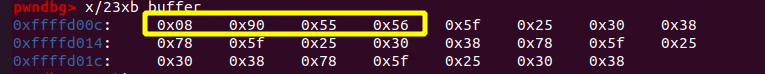
\includegraphics[width=\linewidth]{imgs/format_strings/fmt_str_arbitrary_read_1.png}
    \caption{Address of \texttt{s3cr3t} on the input buffer}
    \label{fig:fmt_str_arbitrary_read_1}
\end{figure}

The next \texttt{"\%s"} will read the address and treat as a pointer, dereferencing the address and printing the value.

\begin{figure}[H]
    \centering
    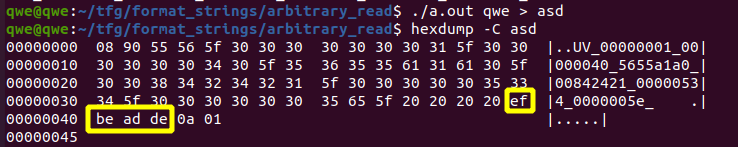
\includegraphics[width=\linewidth]{imgs/format_strings/fmt_str_arbitrary_read_2.png}
    \caption{Value of \texttt{s3cr3t} leaked}
    \label{fig:fmt_str_arbitrary_read_2}
\end{figure}

\subsection{Arbitrary write}
We can employ the same technique from the arbitrary read to overwrite arbitrary memory but instead of using the \texttt{\%s} specifier we use the \texttt{\%n} specifier, which writes back to an address.

The \texttt{\%n} writes the number of bytes written so far. To control that number we can make use of padding and size modifiers.

\subsubsection{Example}
To showcase an arbitrary write from a format string I am going to overwrite the return address without affecting the stack canary. I want to return to the \texttt{win} function that will print out \emph{win} on the screen when executed. This function is called nowhere on the original code. Compile the code with stack canaries enabled.

\begin{figure}[H]
    \centering
    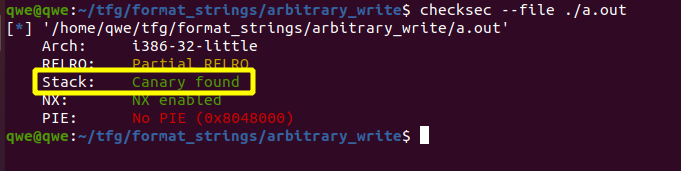
\includegraphics[width=\linewidth]{imgs/format_strings/fmt_str_arbitrary_write_1.png}
    \caption{Compiled with stack canaries}
\end{figure}

Like in the arbitrary read, the first value we put on the input buffer is the address where \texttt{printf} should write to, that is, the address of our return address on the stack. In this particular case I inserted multiple times the address of the buffer in an effort to make the exploit more reliable against stack offsets.
The address is then followed by a pad of format specifiers to align the \texttt{\%n} specifier with the address at the start of the buffer.

Now we need to indicate the value we want to write on the selected address. Because \texttt{\%n} writes back the number of characters already printed, we can use padding in one of the format specifiers to make it print $x$ characters. The address of \texttt{win} is \texttt{0x8049256}. To write that value with \texttt{\%n}, \texttt{printf} needs to print $134517334$ characters minus the previously printed, like the address and the padding format specifiers.

After the calculation, the number of characters left to print is $134517192$.

\lstinputlisting[language=python, caption={exploit.py}]{../../src/format_strings/arbitrary_write/exploit.py}

It is important to \textbf{unset certain environment variables} that could move the stack up and down and make the exploit inconsistent. Running the exploit we execute \texttt{win()}.

\begin{figure}[H]
    \centering
    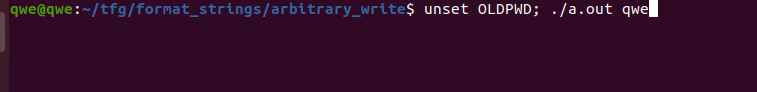
\includegraphics[width=\linewidth]{imgs/format_strings/fmt_str_arbitrary_write_3.png}
    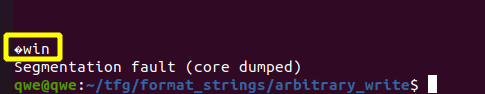
\includegraphics[width=\linewidth]{imgs/format_strings/fmt_str_arbitrary_write_2.png}
    \caption{\texttt{win()} function executed.}
    \label{fig:fmt_str_arbitrary_write_2}
\end{figure}

\end{document}

